\documentclass[11pt,a4paper]{article}
\usepackage[utf8]{inputenc}
\usepackage[T1]{fontenc}
\usepackage[brazilian]{babel}
\usepackage{amsmath,amssymb}
\usepackage{graphicx}
\usepackage{booktabs}
\usepackage{float}
\usepackage{subcaption}
\usepackage[margin=2.2cm]{geometry}
\usepackage[hidelinks]{hyperref}

\begin{document}

\begin{center}
{\LARGE\bfseries Projeto 2: Quantização de Cores com Redes SOM e GNG}\\[6pt]
{\large Disciplina: Introdução às Redes Neurais Artificiais}\\[4pt]
\textbf{Autora:} Aline Breda Kuster (RA: 168.495)\\[2pt]
\textbf{Repositório:} \href{https://github.com/aline-kuster/Proj2}{\texttt{https://github.com/aline-kuster/Proj2}}
\end{center}
\vspace{-4pt}
\noindent\rule{\linewidth}{0.4pt}

\subsection*{Configuração Experimental}

O objetivo é reduzir a paleta de cores de uma imagem (compressão) usando dois modelos de
aprendizado competitivo não supervisionado: o \emph{Self-Organizing Map} (SOM) e o
\emph{Growing Neural Gas} (GNG). Cada pixel é tratado como um vetor $\mathbf{x}=(R,G,B)\in[0,1]^3$;
ao final do treino, os pesos dos neurônios formam a paleta, e a imagem é reconstruída trocando
cada pixel pela cor do neurônio vencedor (BMU):
\begin{equation}
c(\mathbf{x}) = \arg\min_i \|\mathbf{x}-\mathbf{w}_i\|_2 .
\end{equation}

Foram usadas cinco imagens (diretório \texttt{data/input/}), redimensionadas com filtro Lanczos
para no máximo $450$ pixels de lado ($\approx 135\,000$ pixels cada), com semente aleatória fixa em 42:

\begin{table}[H]
\centering\small
\begin{tabular}{llr}
\toprule
Imagem & Conteúdo & Cores distintas \\
\midrule
\texttt{por\_do\_sol} & degradê laranja e silhuetas escuras & $36\,390$ \\
\texttt{campo}        & céu azul, nuvens brancas e grama     & $38\,124$ \\
\texttt{praia}        & céu, mar verde-azulado e areia       & $61\,180$ \\
\texttt{tintas}       & tintas de todas as cores (arco-íris) & $92\,991$ \\
\texttt{arara}        & arara azul e amarela, fundo desfocado & $78\,855$ \\
\bottomrule
\end{tabular}
\caption{Imagens utilizadas.}
\end{table}

Foram avaliadas redes com $16$, $64$ e $256$ neurônios (no SOM, grades $4\times4$, $8\times8$ e
$16\times16$), com quatro métricas:
\begin{enumerate}
  \item \textbf{Erro de Quantização (EQ):} distância média entre cada pixel e a cor do seu BMU;
  \item \textbf{Erro Topológico (ET):} fração de pixels cujo 1º e 2º BMU \emph{não} são vizinhos
        na rede (no SOM, adjacentes na grade; no GNG, ligados por aresta);
  \item \textbf{PSNR (dB):} qualidade visual da imagem reconstruída, $10\log_{10}(255^2/\text{MSE})$;
  \item \textbf{Cores usadas:} quantos neurônios viraram a cor de algum pixel.
\end{enumerate}

\paragraph{Ajuste de hiperparâmetros.} Para cada tamanho de rede foram testadas três
configurações (Tabela~\ref{tab:cfg}); nas tabelas e figuras a seguir é usada a de menor EQ.

\begin{table}[H]
\centering\small
\begin{tabular}{lll}
\toprule
Config. & SOM & GNG \\
\midrule
A & $\sigma_0=L/2$, $\sigma_N=1{,}0$ & $\varepsilon_b=0{,}2$, $\varepsilon_n=0{,}006$, $\lambda=100$, $a_{\max}=50$ \\
B & $\sigma_0=L/2$, $\sigma_N=0{,}5$ & $\varepsilon_b=0{,}05$, $\varepsilon_n=0{,}0006$, $\lambda=100$, $a_{\max}=50$ \\
C & $\sigma_0=L/4$, $\sigma_N=1{,}0$ & $\varepsilon_b=0{,}2$, $\varepsilon_n=0{,}006$, $\lambda=300$, $a_{\max}=100$ \\
\bottomrule
\end{tabular}
\caption{Configurações testadas ($L$ = lado da grade).}
\label{tab:cfg}
\end{table}

\section*{1. Mapas Auto-Organizáveis (SOM)}

O SOM foi treinado com a biblioteca \emph{XPySom} por 100 épocas (todos os pixels a cada época),
com pesos iniciais sorteados entre os pixels e vizinhança gaussiana cujo raio $\sigma$ decai
exponencialmente de $\sigma_0$ até $\sigma_N$. A XPySom usa o \emph{batch SOM}, em que cada peso é
substituído pela média dos pixels ponderada pela vizinhança; nessa conta a taxa de aprendizado
se cancela, por isso o ajuste foi feito no raio $\sigma$. O projeto também traz uma implementação
própria do SOM online (\texttt{--som-impl propria}).

\begin{table}[H]
\centering\small
\begin{tabular}{llcccccc}
\toprule
Imagem & Grade & Config. & EQ & ET & PSNR (dB) & Cores \\
\midrule
\texttt{por\_do\_sol} & 4x4 & B & 0{,}0307 & 0{,}0000 & 33{,}39 & 16 \\
\texttt{por\_do\_sol} & 8x8 & B & 0{,}0158 & 0{,}1510 & 39{,}01 & 64 \\
\texttt{por\_do\_sol} & 16x16 & B & 0{,}0086 & 0{,}2063 & 44{,}23 & 255 \\
\midrule
\texttt{campo} & 4x4 & B & 0{,}0421 & 0{,}0068 & 30{,}58 & 15 \\
\texttt{campo} & 8x8 & B & 0{,}0183 & 0{,}0553 & 37{,}28 & 62 \\
\texttt{campo} & 16x16 & B & 0{,}0098 & 0{,}1652 & 43{,}12 & 254 \\
\midrule
\texttt{praia} & 4x4 & B & 0{,}0521 & 0{,}0466 & 29{,}16 & 16 \\
\texttt{praia} & 8x8 & B & 0{,}0257 & 0{,}0661 & 35{,}14 & 64 \\
\texttt{praia} & 16x16 & B & 0{,}0145 & 0{,}0697 & 39{,}95 & 256 \\
\midrule
\texttt{tintas} & 4x4 & B & 0{,}1075 & 0{,}1017 & 22{,}84 & 16 \\
\texttt{tintas} & 8x8 & B & 0{,}0534 & 0{,}0901 & 28{,}93 & 64 \\
\texttt{tintas} & 16x16 & B & 0{,}0295 & 0{,}1264 & 33{,}84 & 245 \\
\midrule
\texttt{arara} & 4x4 & B & 0{,}0730 & 0{,}0234 & 26{,}21 & 16 \\
\texttt{arara} & 8x8 & B & 0{,}0373 & 0{,}0198 & 31{,}85 & 64 \\
\texttt{arara} & 16x16 & B & 0{,}0213 & 0{,}1770 & 36{,}44 & 256 \\
\midrule
\textbf{Média} & 4x4 & -- & 0{,}0611 & 0{,}0357 & 28{,}44 & 15{,}8 \\
\textbf{Média} & 8x8 & -- & 0{,}0301 & 0{,}0765 & 34{,}44 & 63{,}6 \\
\textbf{Média} & 16x16 & -- & 0{,}0167 & 0{,}1489 & 39{,}51 & 253{,}2 \\
\bottomrule
\end{tabular}

\caption{Métricas do SOM (melhor configuração de cada grade).}
\label{tab:som}
\end{table}

Dobrar o lado da grade reduz o erro de quantização aproximadamente pela metade, e o PSNR médio
sobe de $28{,}4$ dB (16 cores) para $34{,}4$ dB (64) e $39{,}5$ dB (256). Com 16 cores aparecem
faixas (posterização) nos degradês; com 256 a reconstrução é praticamente igual à original. Já o
erro topológico \emph{aumenta} com a grade (média de $0{,}036$ para $0{,}149$): quanto mais
neurônios, mais a grade 2D precisa se dobrar para cobrir a nuvem de cores 3D. Em compensação, a
paleta do SOM sai organizada, com cores parecidas lado a lado (Figura~\ref{fig:som-por}).

\begin{figure}[H]
\centering
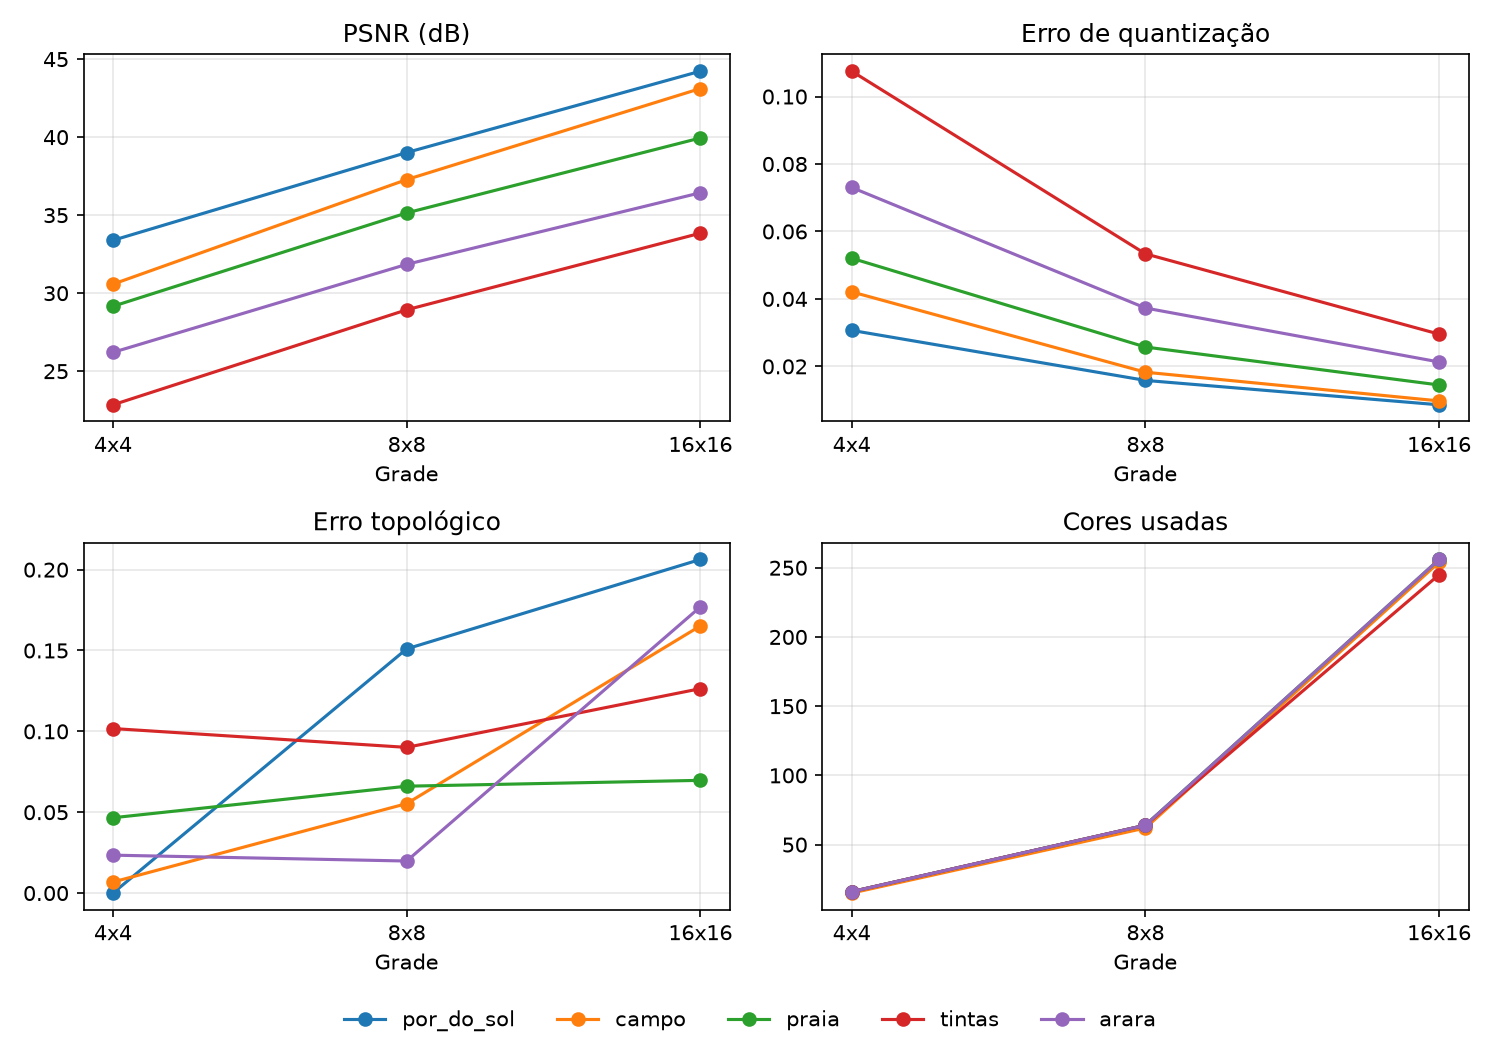
\includegraphics[width=0.92\linewidth]{figures/som_curvas.png}
\caption{Desempenho do SOM em função do tamanho da grade, nas cinco imagens.}
\end{figure}

\begin{figure}[H]
\centering
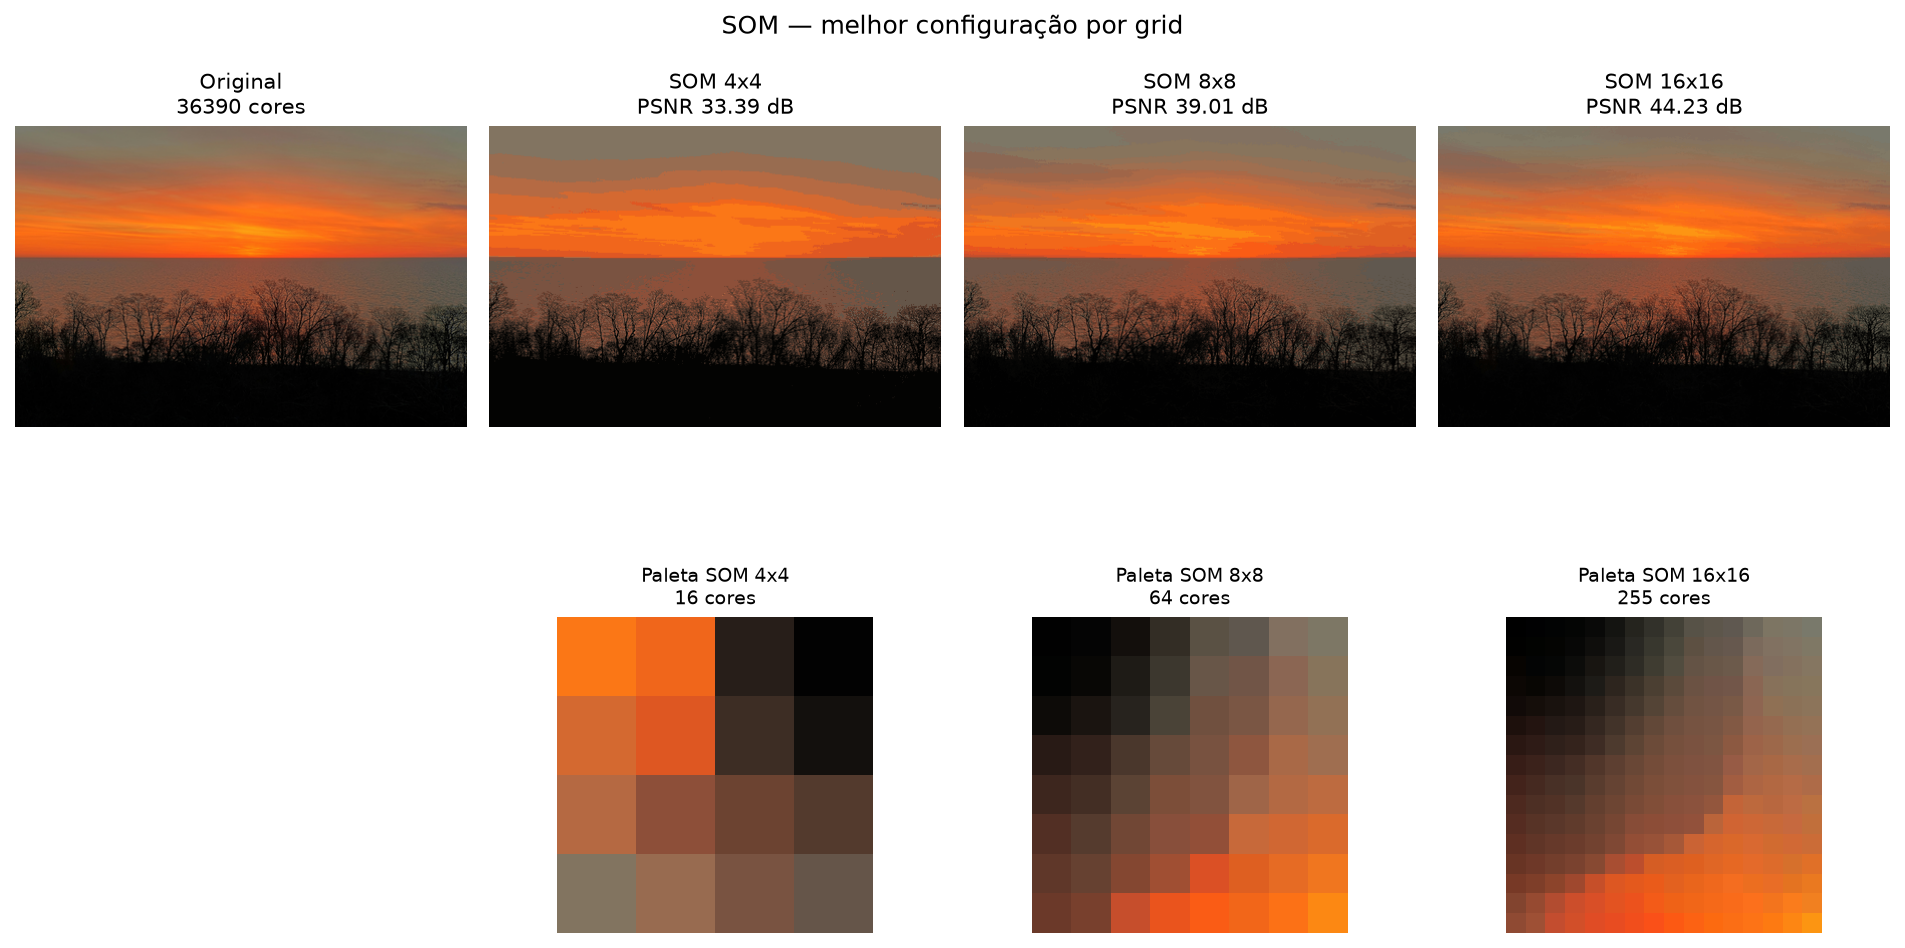
\includegraphics[width=\linewidth]{figures/por_do_sol/som_grade.png}
\caption{SOM no \texttt{por\_do\_sol}: reconstruções e paletas (na posição da grade).}
\label{fig:som-por}
\end{figure}

\begin{figure}[H]
\centering
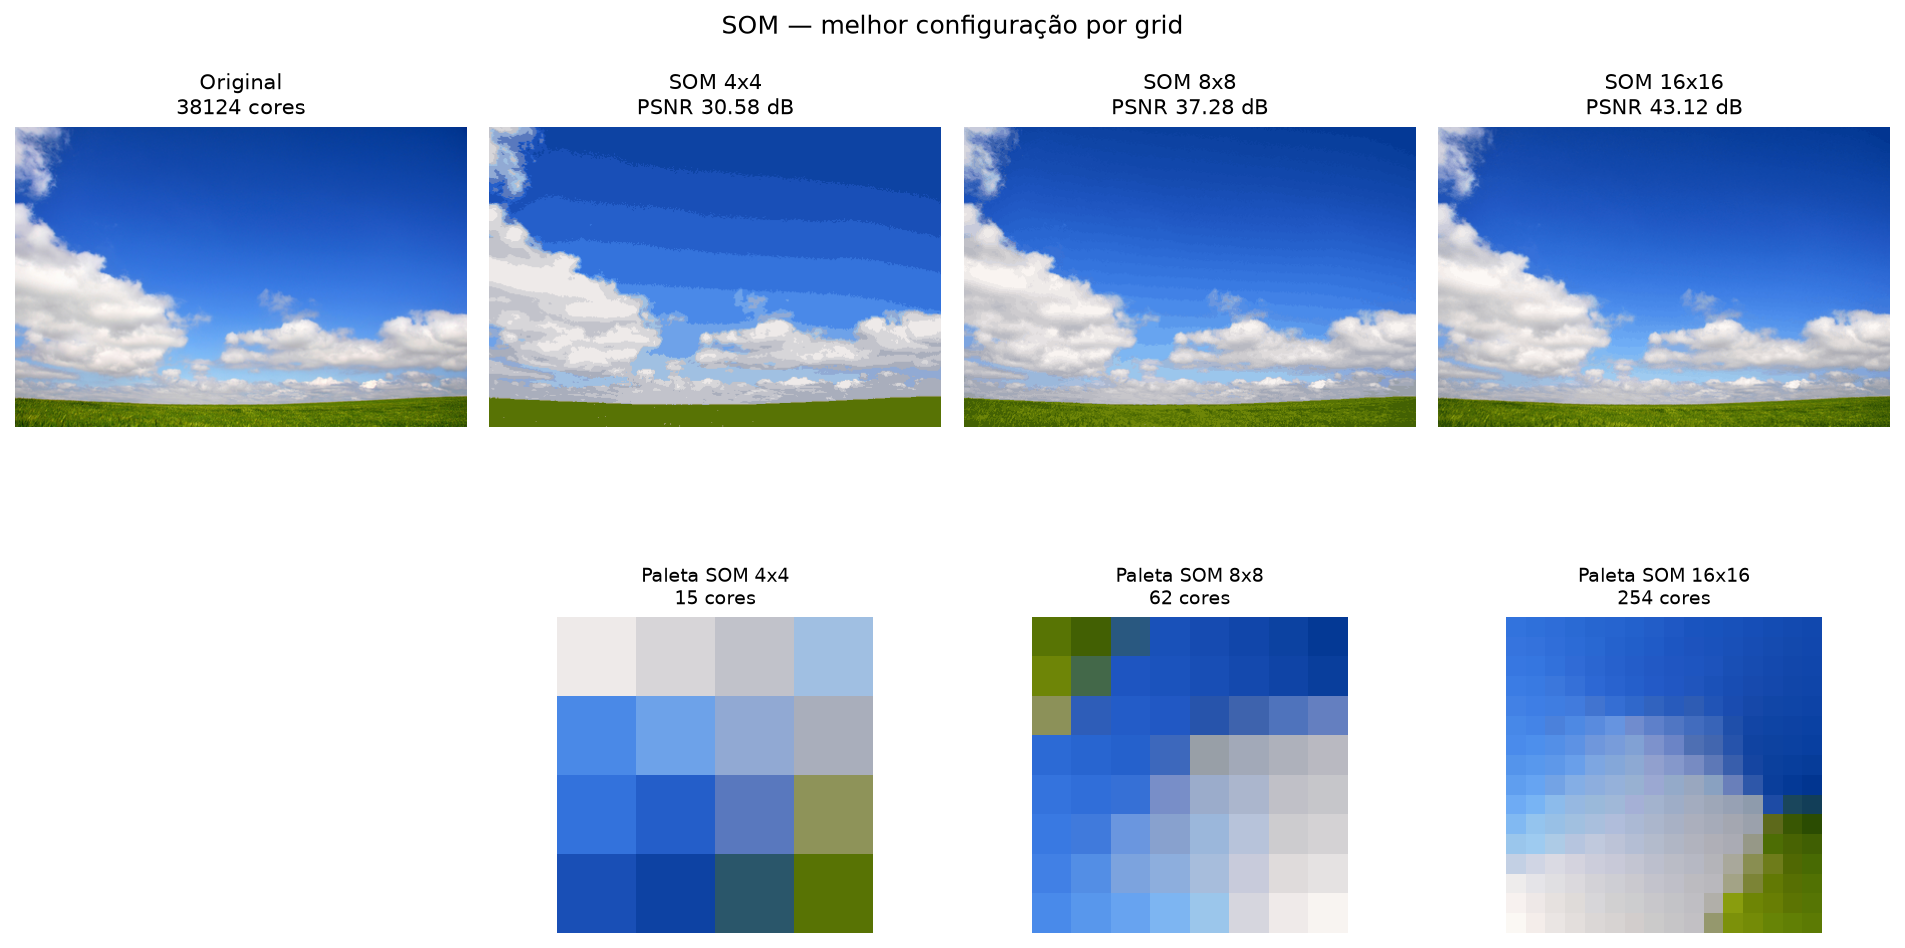
\includegraphics[width=\linewidth]{figures/campo/som_grade.png}
\caption{SOM no \texttt{campo}.}
\end{figure}

\begin{figure}[H]
\centering
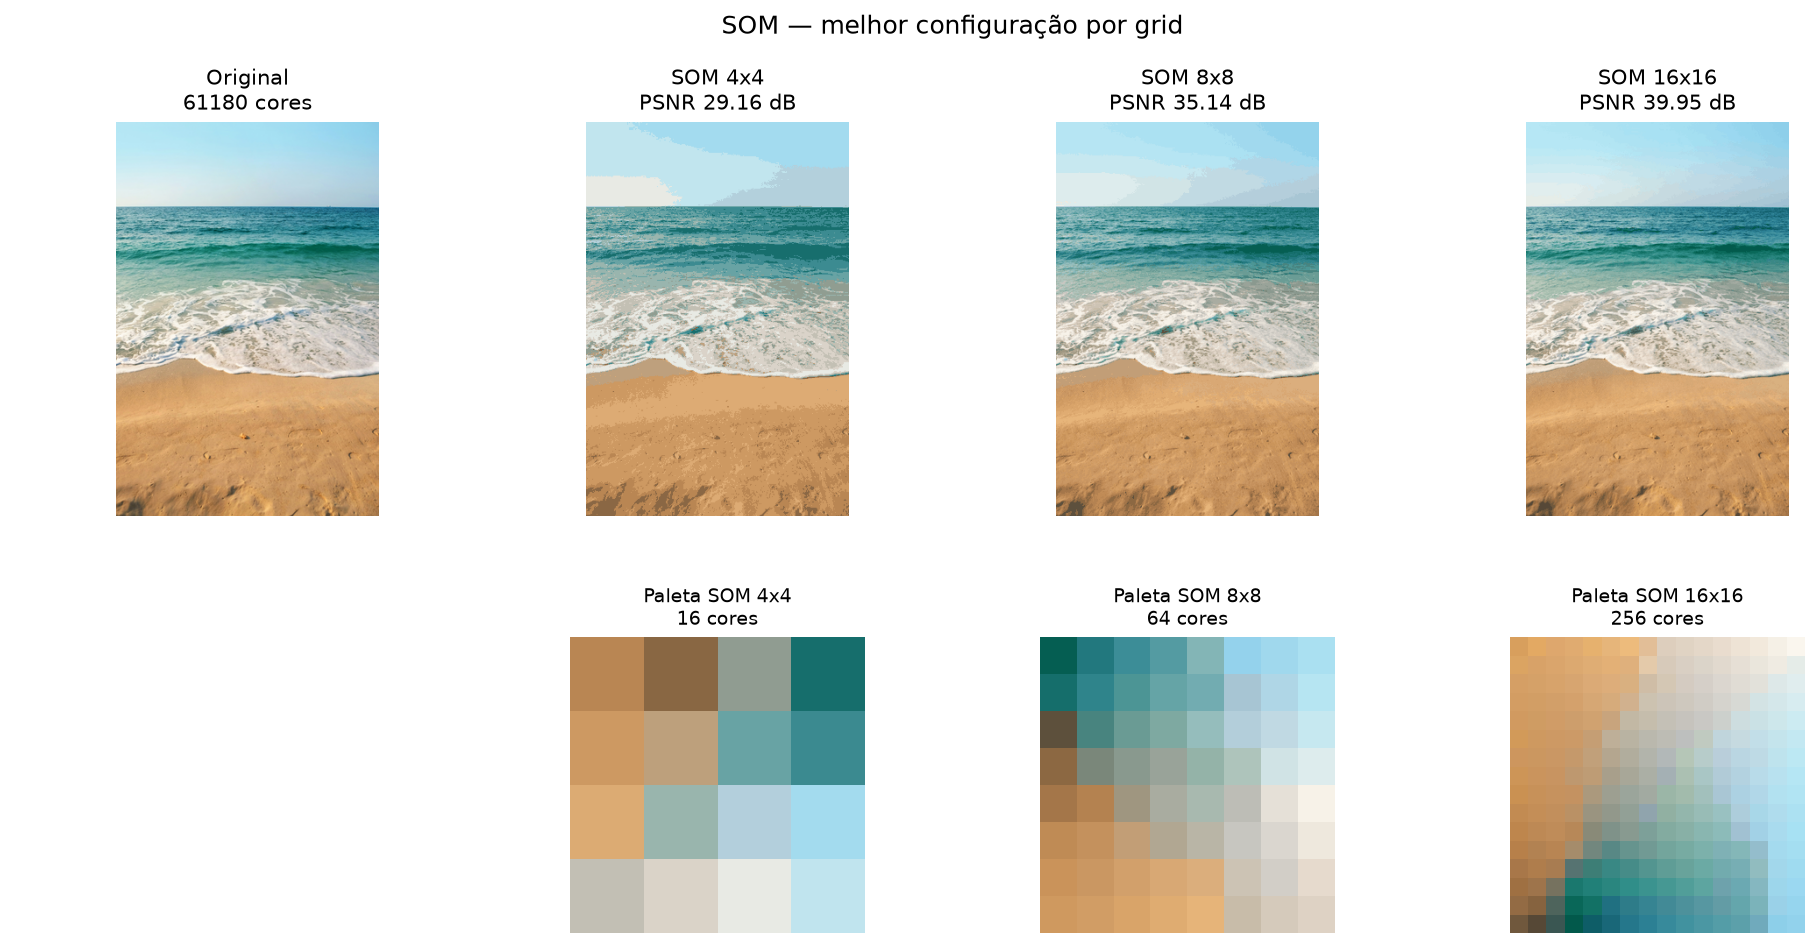
\includegraphics[width=\linewidth]{figures/praia/som_grade.png}
\caption{SOM na \texttt{praia}.}
\end{figure}

\begin{figure}[H]
\centering
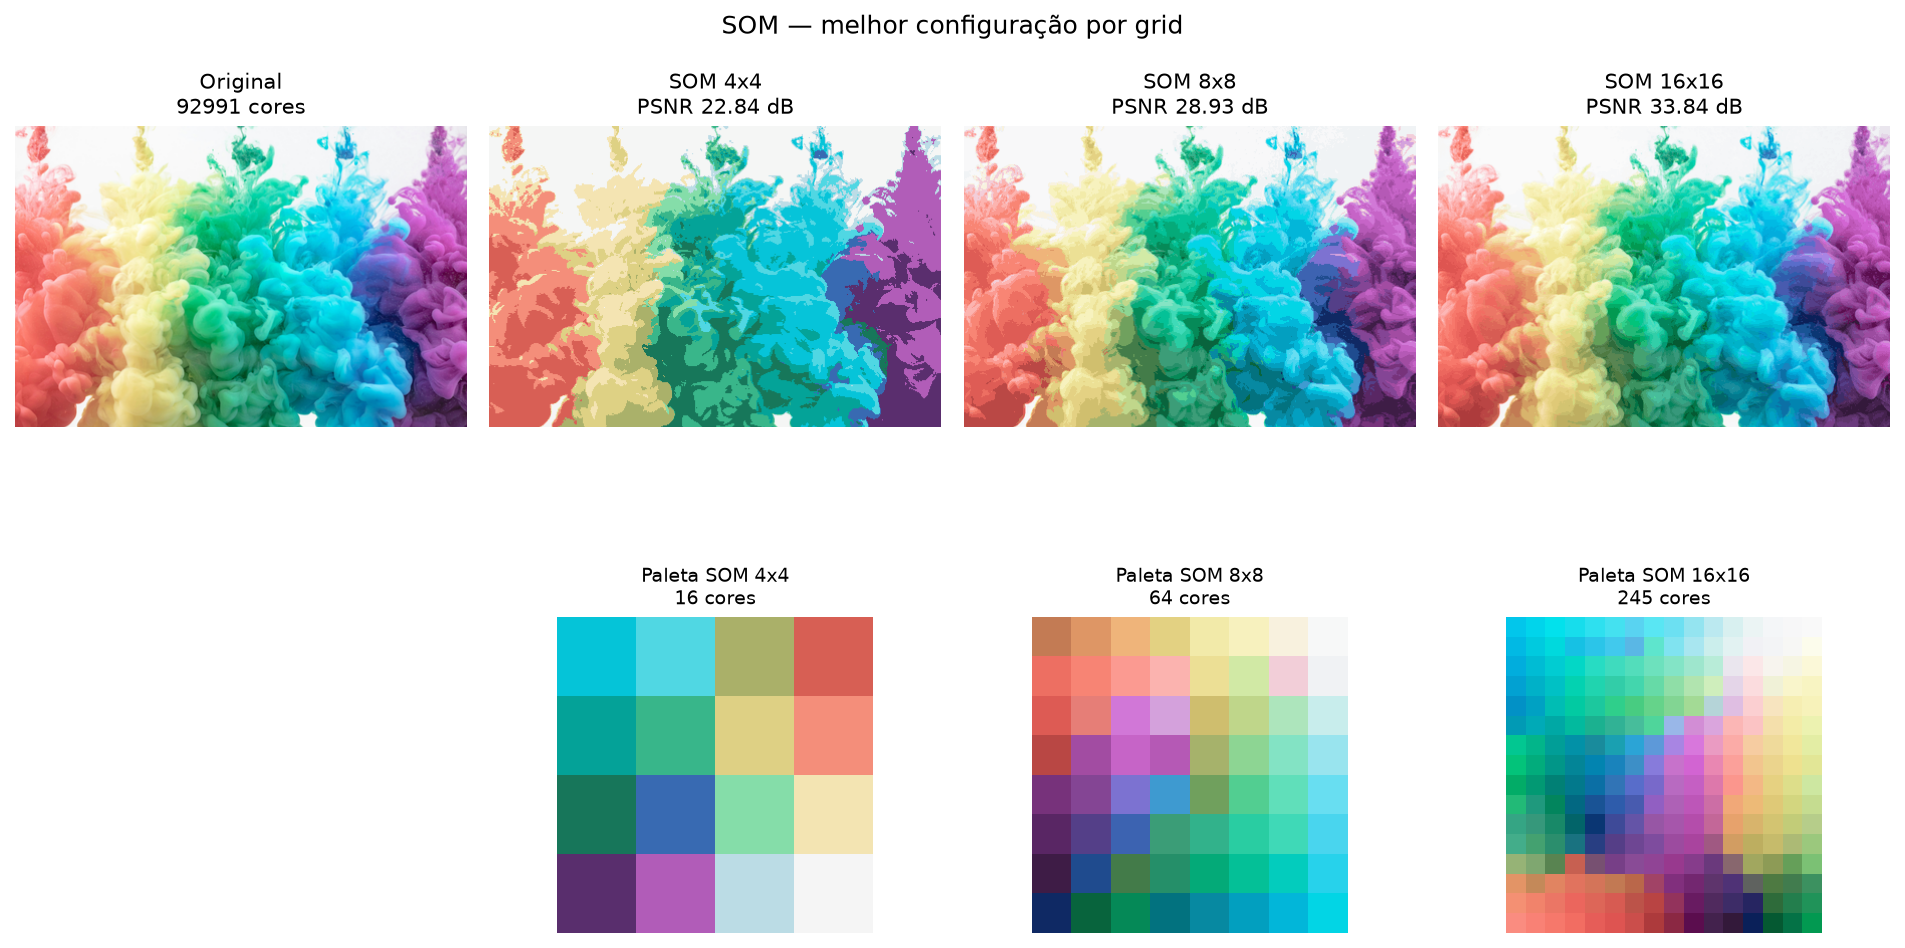
\includegraphics[width=\linewidth]{figures/tintas/som_grade.png}
\caption{SOM nas \texttt{tintas}, a imagem mais difícil (cores espalhadas por todo o cubo RGB).}
\end{figure}

\begin{figure}[H]
\centering
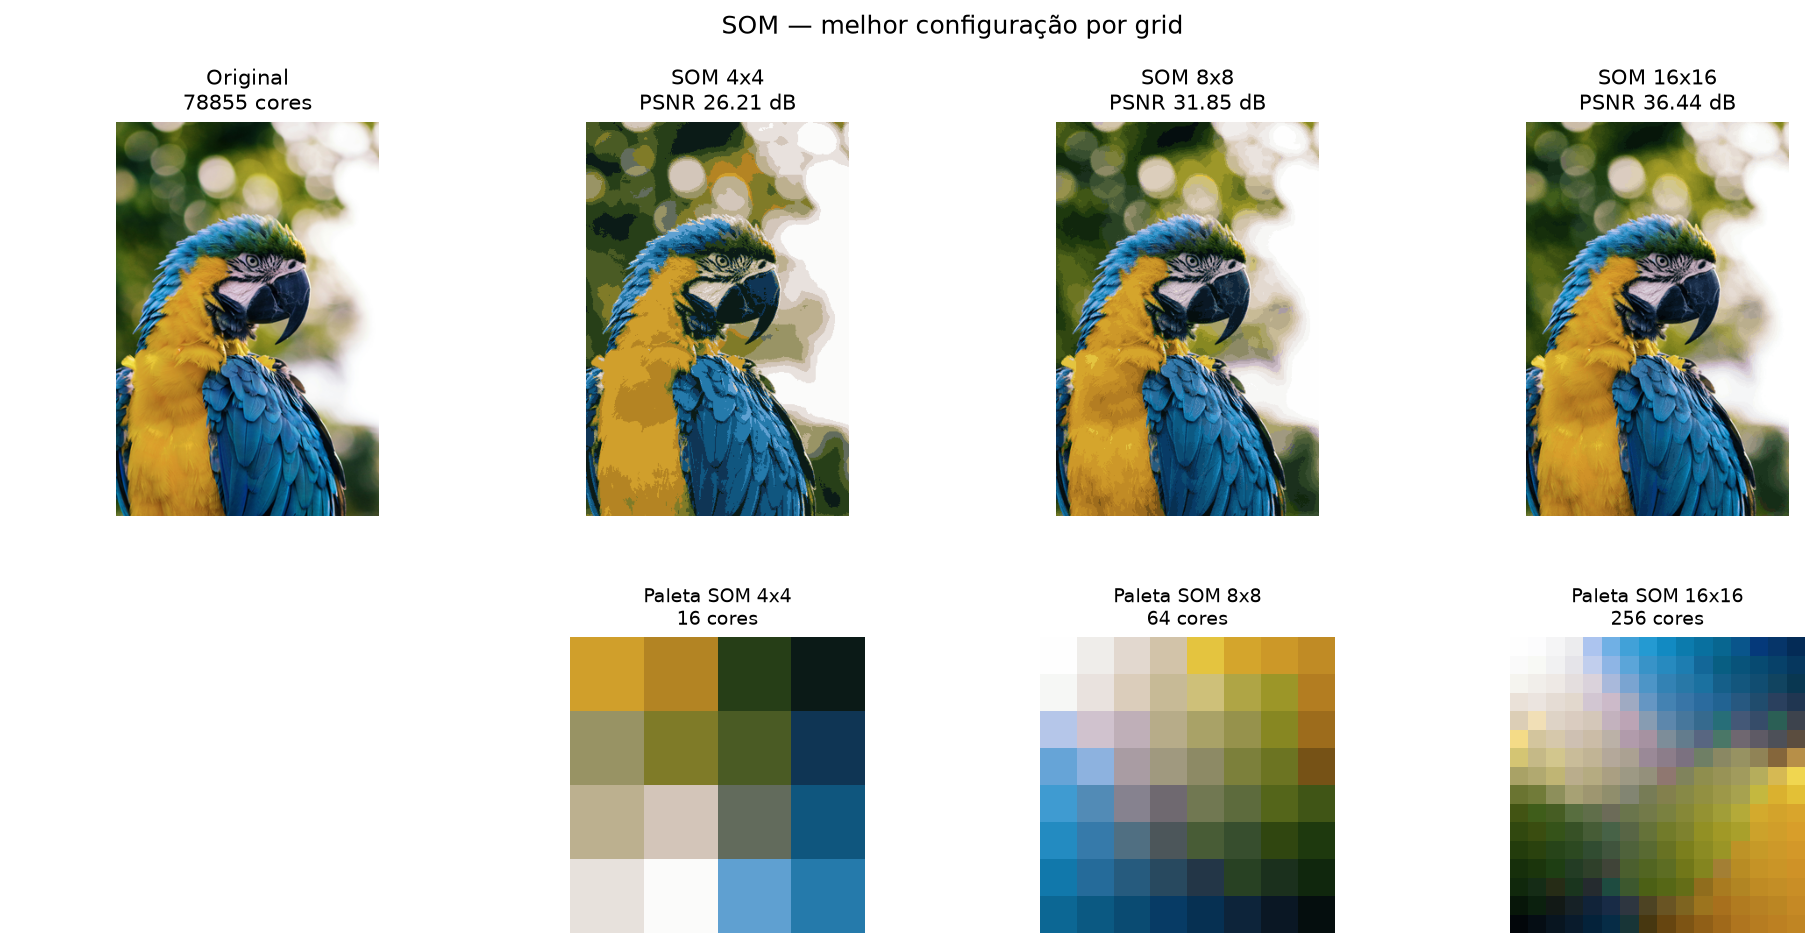
\includegraphics[width=\linewidth]{figures/arara/som_grade.png}
\caption{SOM na \texttt{arara}.}
\end{figure}

\section*{2. Growing Neural Gas (GNG)}

O GNG foi implementado do zero (Fritzke, 1995). A rede começa com 2 neurônios; a cada pixel, o
vencedor $s_1$ e seus vizinhos são movidos em direção à amostra (taxas $\varepsilon_b$ e
$\varepsilon_n$), a aresta $s_1$--$s_2$ é criada ou renovada, e arestas com idade maior que
$a_{\max}$ são removidas. A cada $\lambda$ iterações é inserido um neurônio entre o de maior erro
acumulado e seu vizinho de maior erro ($\alpha=0{,}5$, $d=0{,}995$). O treino dura 2 épocas
($\approx 270\,000$ iterações): primeiro a rede cresce até o tamanho final e depois faz o ajuste fino.

\begin{table}[H]
\centering\small
\begin{tabular}{llcccccc}
\toprule
Imagem & Neurônios & Config. & EQ & ET & PSNR (dB) & Cores \\
\midrule
\texttt{por\_do\_sol} & 16 & B & 0{,}0308 & 0{,}0011 & 33{,}31 & 16 \\
\texttt{por\_do\_sol} & 64 & B & 0{,}0156 & 0{,}0016 & 39{,}29 & 64 \\
\texttt{por\_do\_sol} & 256 & C & 0{,}0085 & 0{,}0041 & 44{,}12 & 256 \\
\midrule
\texttt{campo} & 16 & B & 0{,}0395 & 0{,}0028 & 31{,}17 & 16 \\
\texttt{campo} & 64 & A & 0{,}0178 & 0{,}0030 & 37{,}86 & 64 \\
\texttt{campo} & 256 & A & 0{,}0101 & 0{,}0089 & 43{,}01 & 256 \\
\midrule
\texttt{praia} & 16 & B & 0{,}0517 & 0{,}0036 & 29{,}29 & 16 \\
\texttt{praia} & 64 & B & 0{,}0257 & 0{,}0080 & 35{,}36 & 64 \\
\texttt{praia} & 256 & A & 0{,}0152 & 0{,}0090 & 39{,}80 & 256 \\
\midrule
\texttt{tintas} & 16 & B & 0{,}1064 & 0{,}0047 & 23{,}08 & 16 \\
\texttt{tintas} & 64 & B & 0{,}0539 & 0{,}0040 & 28{,}96 & 64 \\
\texttt{tintas} & 256 & B & 0{,}0296 & 0{,}0090 & 34{,}08 & 256 \\
\midrule
\texttt{arara} & 16 & B & 0{,}0751 & 0{,}0119 & 26{,}04 & 16 \\
\texttt{arara} & 64 & B & 0{,}0376 & 0{,}0044 & 31{,}77 & 64 \\
\texttt{arara} & 256 & A & 0{,}0221 & 0{,}0140 & 36{,}10 & 256 \\
\midrule
\textbf{Média} & 16 & -- & 0{,}0607 & 0{,}0048 & 28{,}58 & 16{,}0 \\
\textbf{Média} & 64 & -- & 0{,}0301 & 0{,}0042 & 34{,}65 & 64{,}0 \\
\textbf{Média} & 256 & -- & 0{,}0171 & 0{,}0090 & 39{,}42 & 256{,}0 \\
\bottomrule
\end{tabular}

\caption{Métricas do GNG (melhor configuração de cada tamanho).}
\label{tab:gng}
\end{table}

O PSNR médio do GNG foi de $28{,}6$ dB (16 neurônios), $34{,}7$ dB (64) e $39{,}4$ dB (256), muito
próximo do SOM. A grande diferença está no erro topológico, que ficou sempre abaixo de $0{,}015$
(média de $0{,}004$ a $0{,}009$). Como as arestas ligam exatamente o 1º e o 2º BMU de cada pixel, a
topologia do grafo acompanha a distribuição real das cores (Figura~\ref{fig:topo}). A paleta, por
outro lado, não tem ordem visual, pois os neurônios ficam na ordem em que foram inseridos.

\begin{figure}[H]
\centering
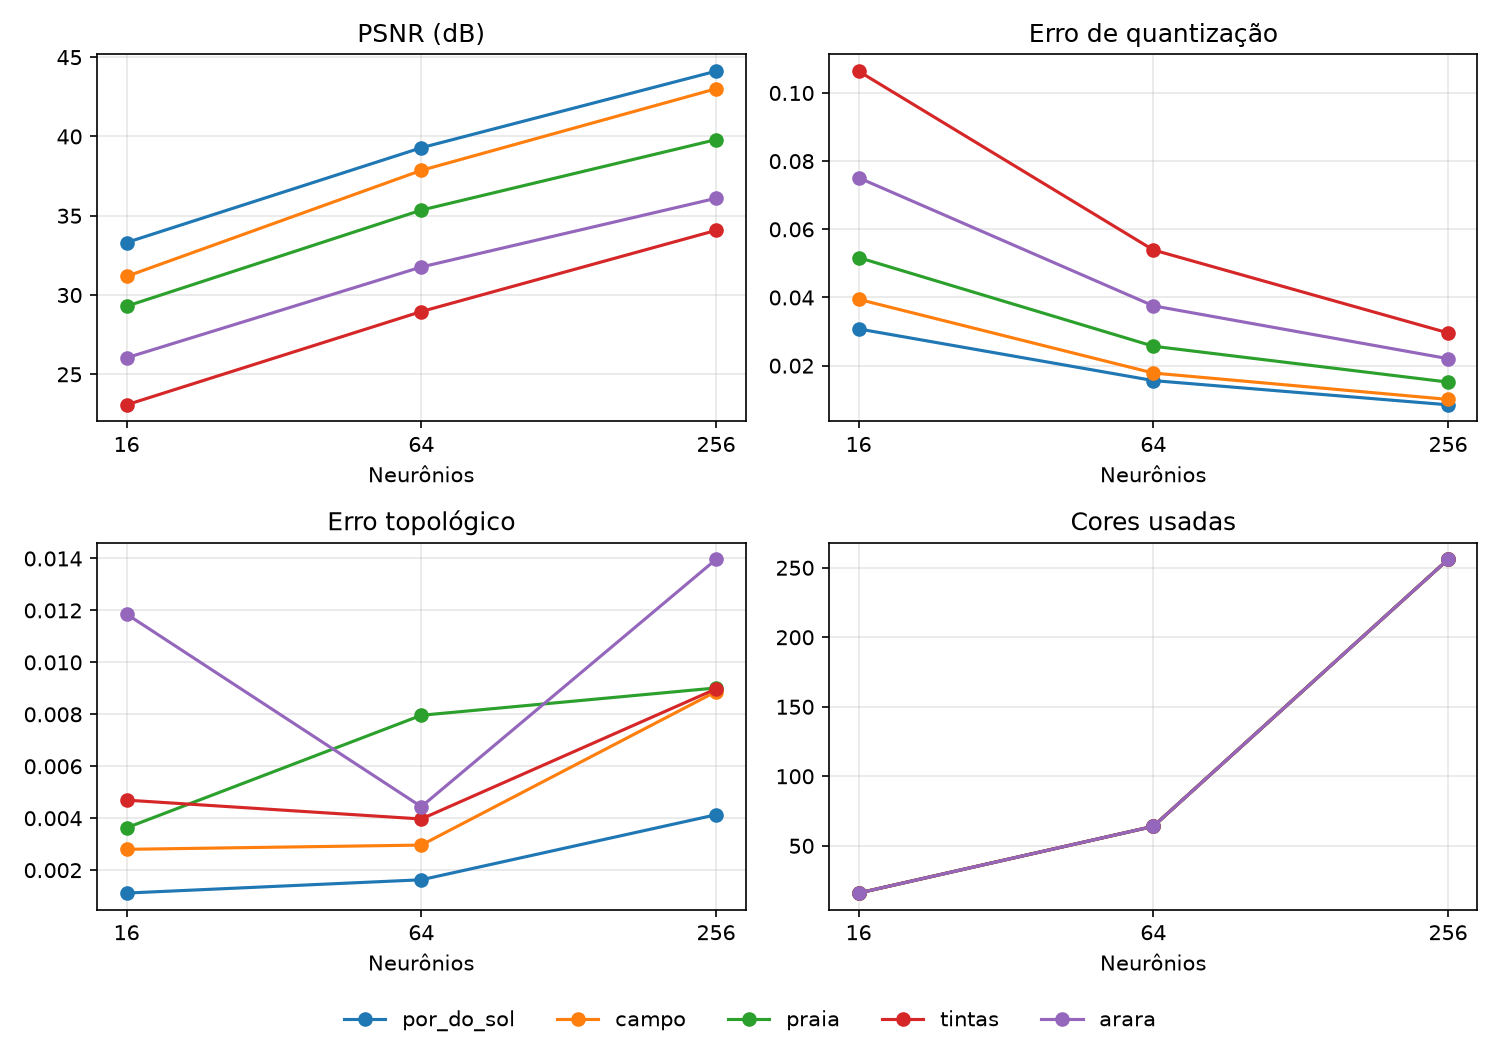
\includegraphics[width=0.92\linewidth]{figures/gng_curvas.png}
\caption{Desempenho do GNG em função do número de neurônios. Atenção à escala do erro
topológico: cerca de 15 vezes menor que a do SOM.}
\end{figure}

\begin{figure}[H]
\centering
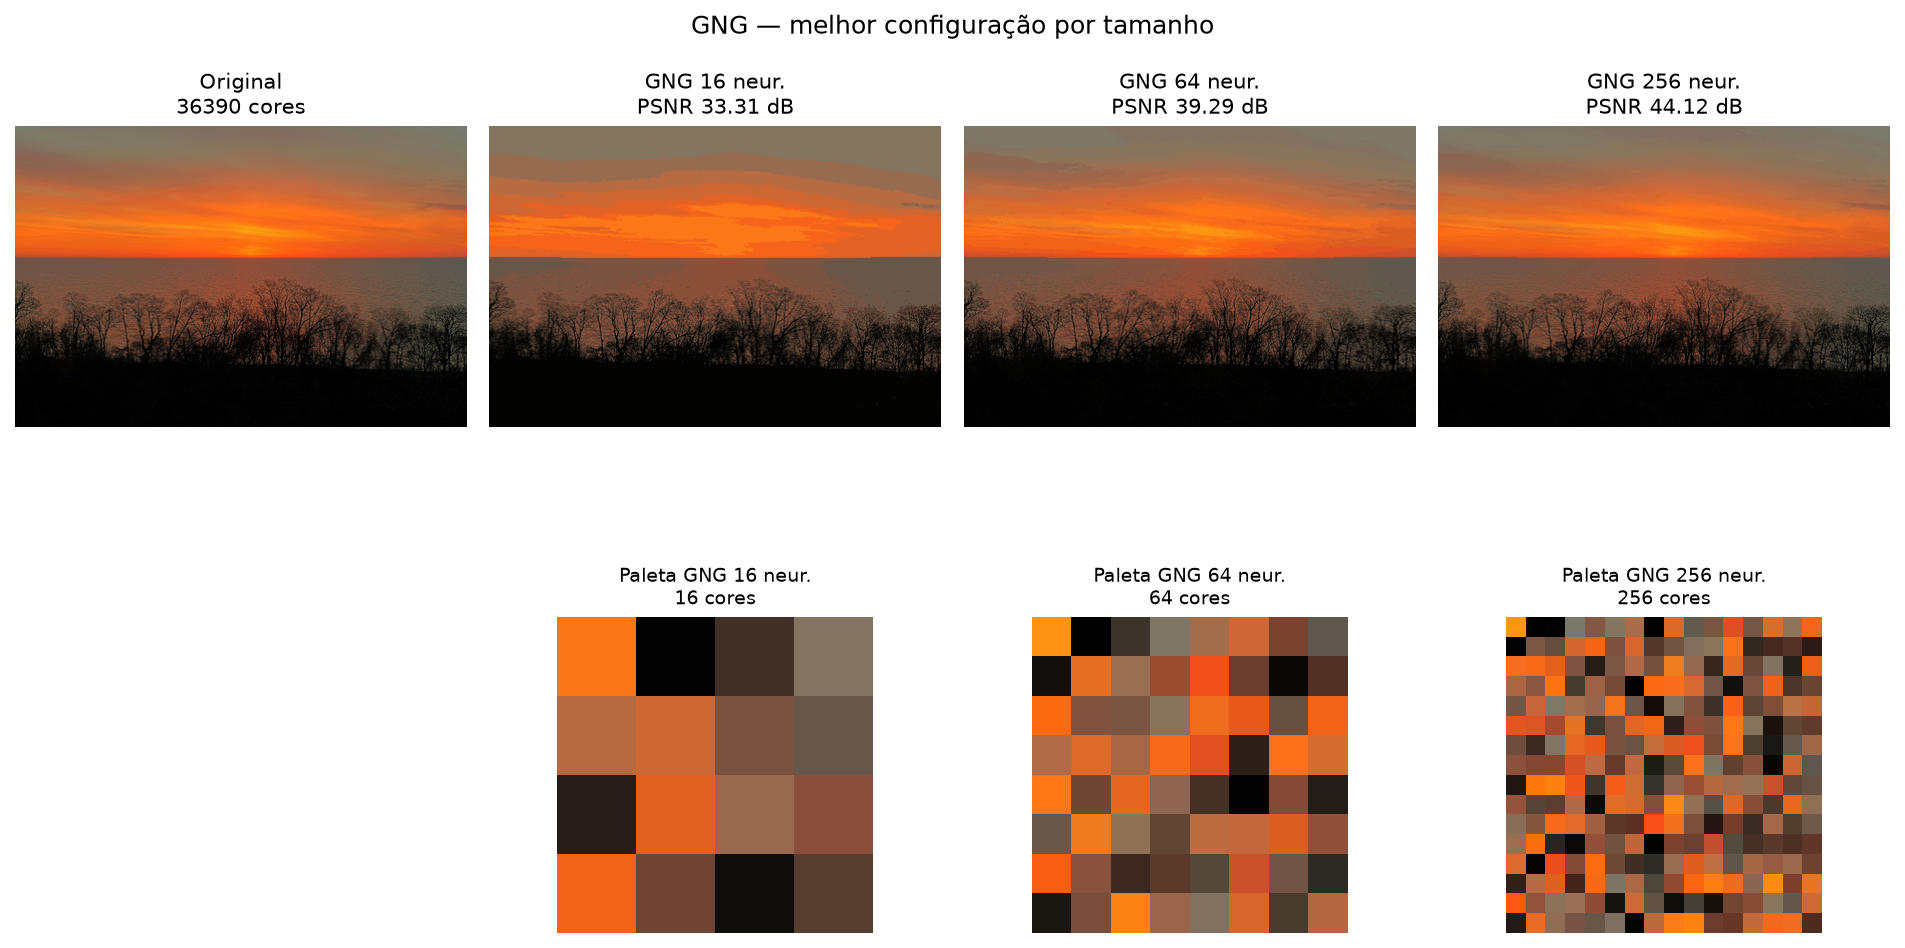
\includegraphics[width=\linewidth]{figures/por_do_sol/gng_grade.png}
\caption{GNG no \texttt{por\_do\_sol}: reconstruções e paletas (na ordem de inserção).}
\end{figure}

\begin{figure}[H]
\centering
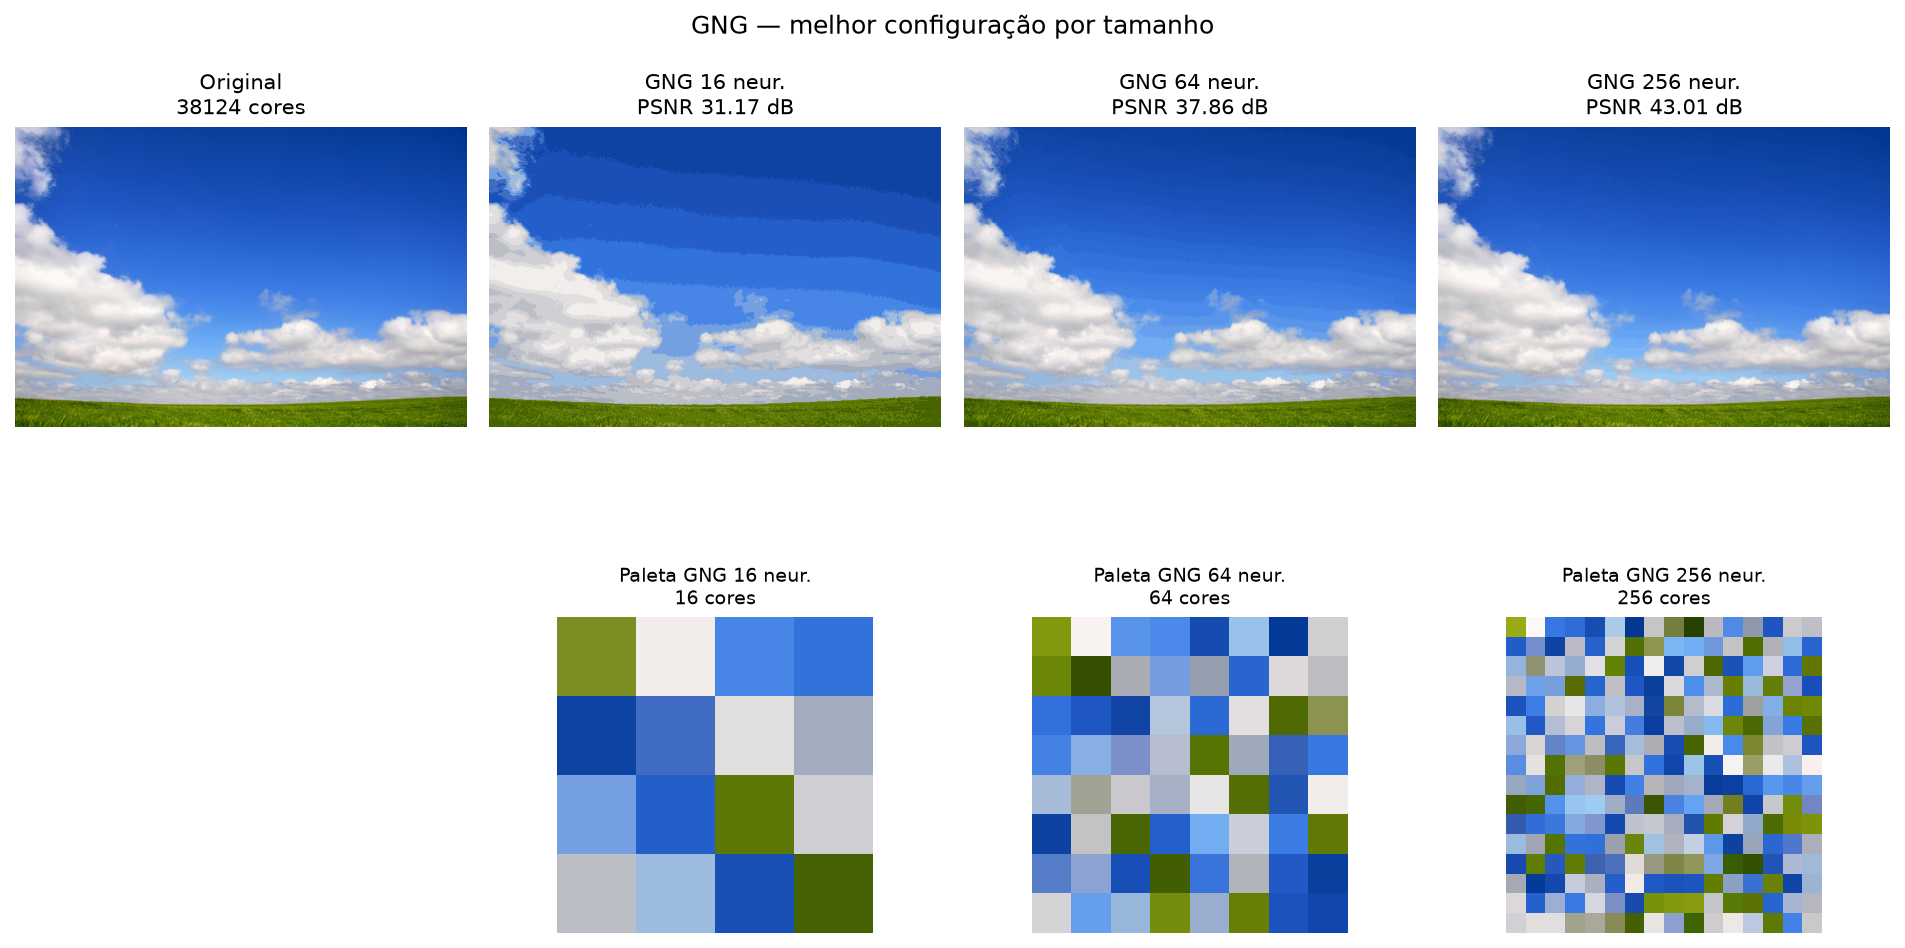
\includegraphics[width=\linewidth]{figures/campo/gng_grade.png}
\caption{GNG no \texttt{campo}.}
\end{figure}

\begin{figure}[H]
\centering
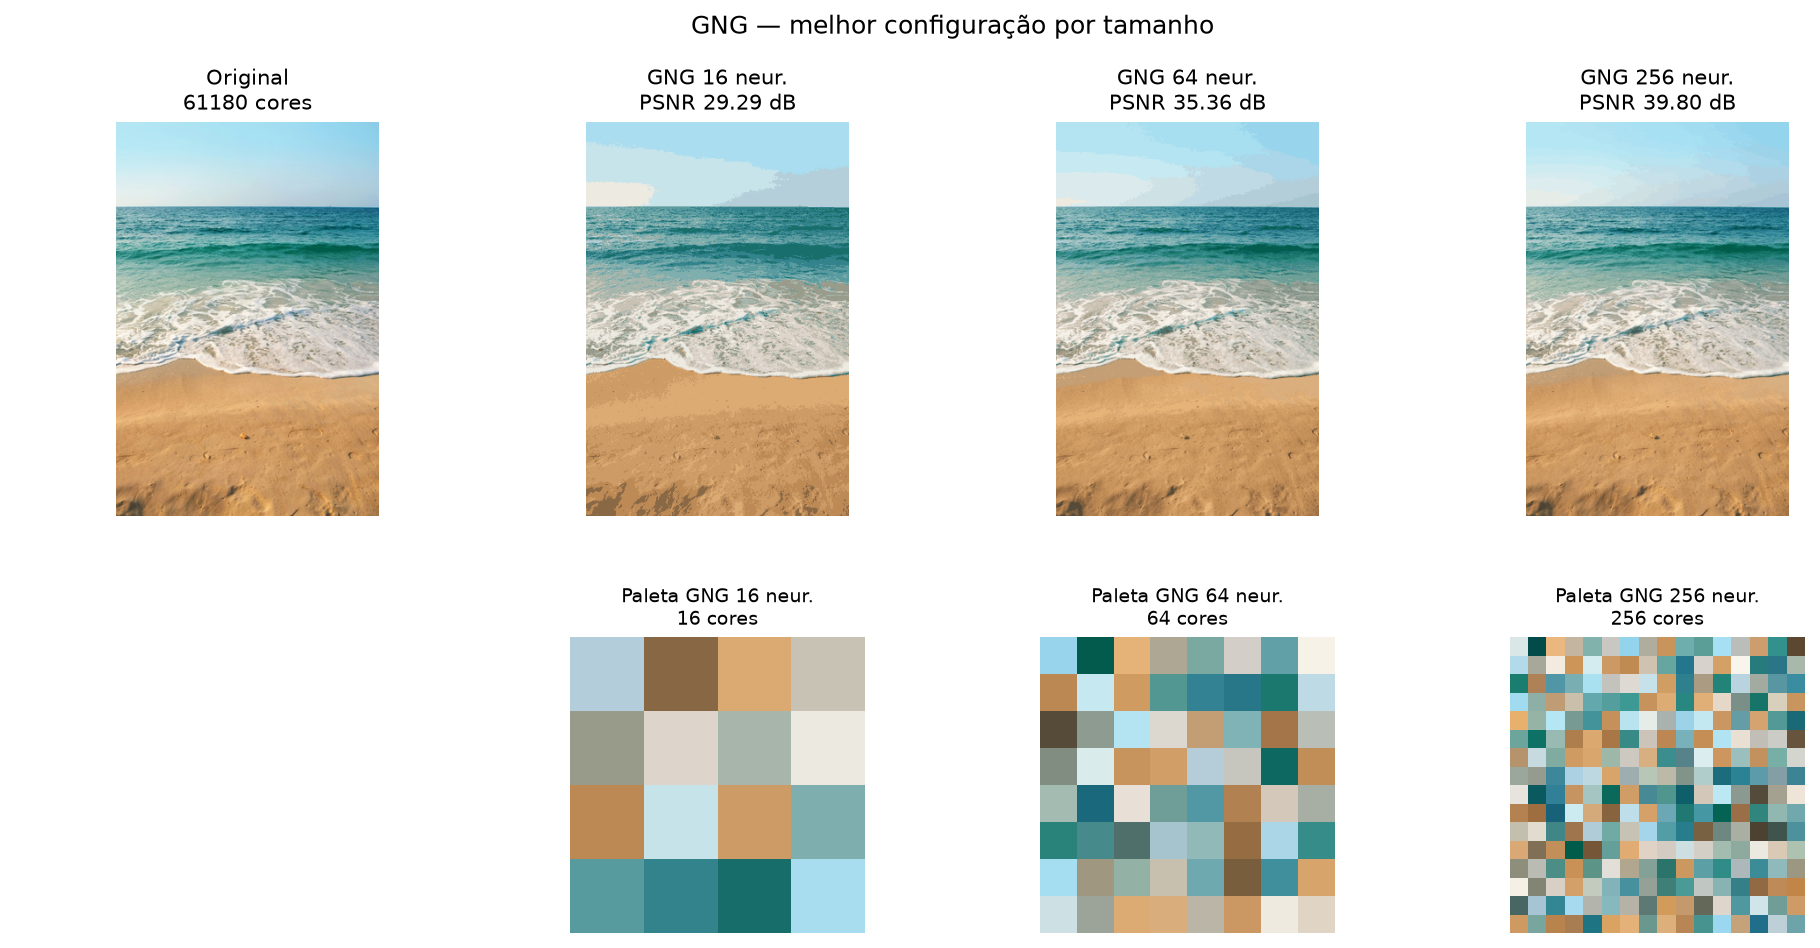
\includegraphics[width=\linewidth]{figures/praia/gng_grade.png}
\caption{GNG na \texttt{praia}.}
\end{figure}

\begin{figure}[H]
\centering
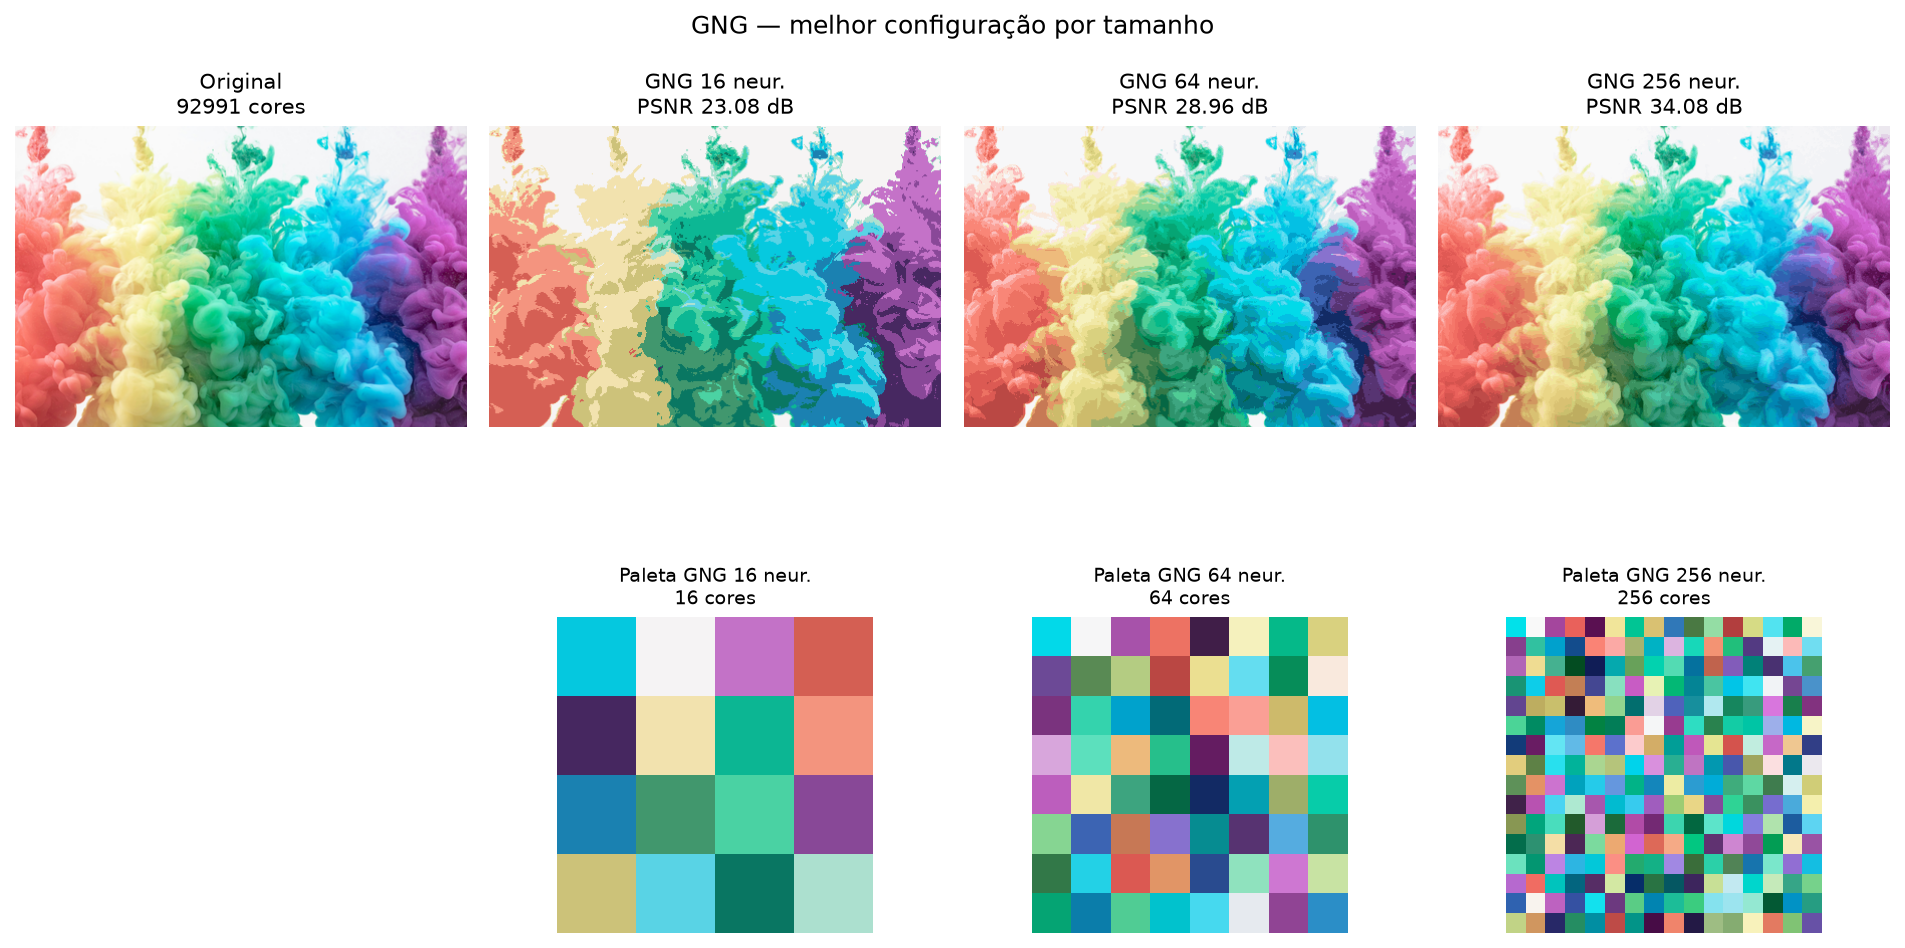
\includegraphics[width=\linewidth]{figures/tintas/gng_grade.png}
\caption{GNG nas \texttt{tintas}.}
\end{figure}

\begin{figure}[H]
\centering
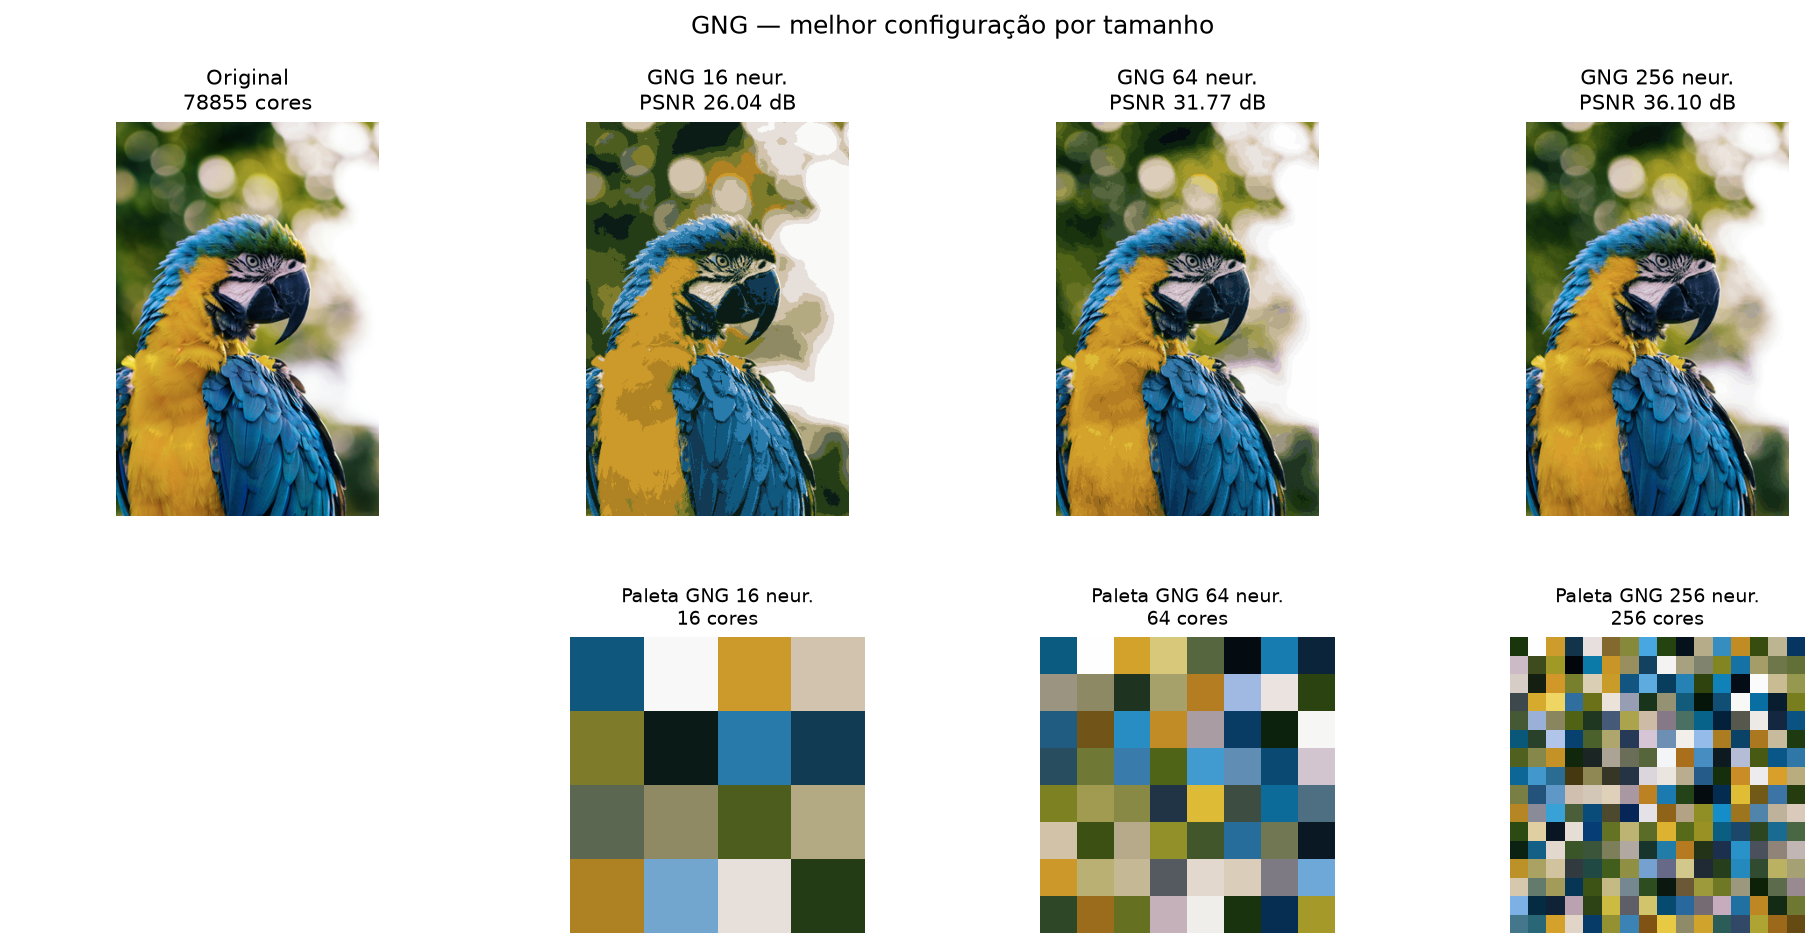
\includegraphics[width=\linewidth]{figures/arara/gng_grade.png}
\caption{GNG na \texttt{arara}.}
\end{figure}

\begin{figure}[H]
\centering
\begin{subfigure}{0.48\linewidth}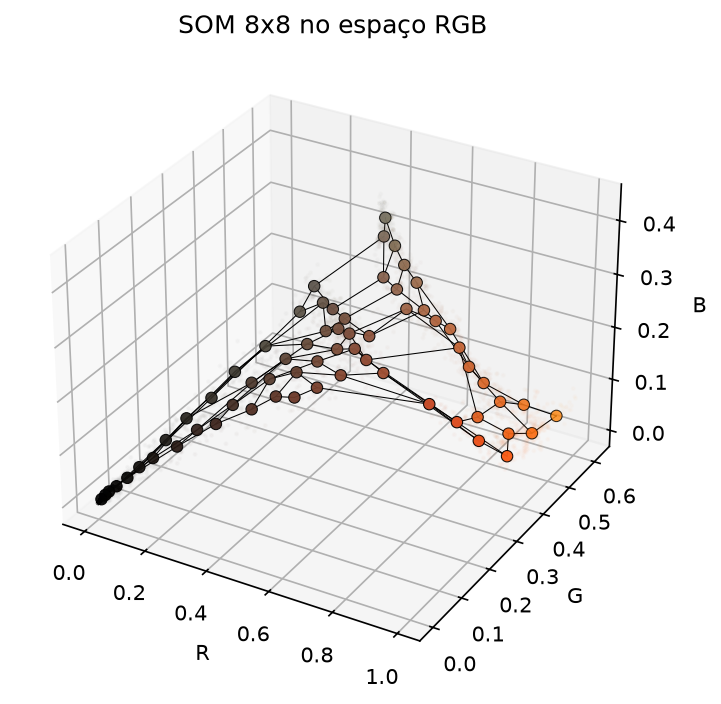
\includegraphics[width=\linewidth]{figures/por_do_sol/som_8x8_rgb.png}
\caption{SOM $8\times8$: a grade se dobra para cobrir as cores.}\end{subfigure}
\hfill
\begin{subfigure}{0.48\linewidth}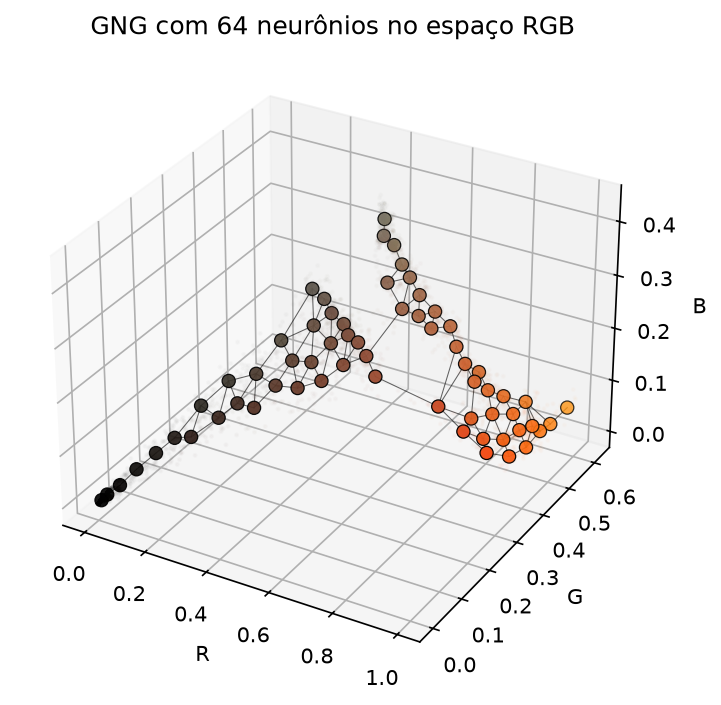
\includegraphics[width=\linewidth]{figures/por_do_sol/gng_64n_rgb.png}
\caption{GNG com 64 neurônios: o grafo segue as cores.}\end{subfigure}
\caption{Topologia das redes no espaço RGB (\texttt{por\_do\_sol}).}
\label{fig:topo}
\end{figure}

\section*{3. Ajuste de Hiperparâmetros}

\begin{table}[H]
\centering\small
\begin{tabular}{llcccc}
\toprule
Modelo & Config. & EQ médio & ET médio & Menor EQ & Menor ET \\
\midrule
SOM & A & 0{,}0413 & 0{,}0526 & 0/15 & 10/15 \\
SOM & B & 0{,}0360 & 0{,}0870 & 15/15 & 2/15 \\
SOM & C & 0{,}0425 & 0{,}1045 & 0/15 & 3/15 \\
\midrule
GNG & A & 0{,}0373 & 0{,}0069 & 4/15 & 1/15 \\
GNG & B & 0{,}0362 & 0{,}0052 & 10/15 & 5/15 \\
GNG & C & 0{,}0375 & 0{,}0038 & 1/15 & 9/15 \\
\bottomrule
\end{tabular}

\caption{Efeito das configurações: médias nas 15 combinações (5 imagens $\times$ 3 tamanhos) e
em quantas delas cada configuração teve o menor erro.}
\label{tab:hiper}
\end{table}

No SOM, a configuração B (vizinhança final menor) teve o menor EQ em todos os 15 casos, mas o
maior ET médio: sem a vizinhança puxando os neurônios, o SOM se comporta como um $k$-means e o mapa
se desorganiza. A A (vizinhança final maior) preserva melhor a topologia, e a C (vizinhança
inicial menor) foi a pior nos dois erros, porque a grade não consegue se desdobrar no início do
treino. No GNG, taxas menores (B) deram o menor EQ na maioria dos casos, e inserir neurônios com
menos frequência (C, $\lambda$ maior) deu o menor ET, pois cada neurônio novo tem mais tempo para
se encaixar antes do próximo.

\section*{4. Análise Comparativa}

\begin{table}[H]
\centering\small
\begin{tabular}{lcccccc}
\toprule
 & \multicolumn{2}{c}{16 protótipos} & \multicolumn{2}{c}{64 protótipos} & \multicolumn{2}{c}{256 protótipos} \\
\cmidrule(lr){2-3}\cmidrule(lr){4-5}\cmidrule(lr){6-7}
Imagem & SOM & GNG & SOM & GNG & SOM & GNG \\
\midrule
\multicolumn{7}{l}{\textit{PSNR (dB) -- quanto maior, melhor}} \\
\texttt{por\_do\_sol} & 33{,}39 & 33{,}31 & 39{,}01 & 39{,}29 & 44{,}23 & 44{,}12 \\
\texttt{campo} & 30{,}58 & 31{,}17 & 37{,}28 & 37{,}86 & 43{,}12 & 43{,}01 \\
\texttt{praia} & 29{,}16 & 29{,}29 & 35{,}14 & 35{,}36 & 39{,}95 & 39{,}80 \\
\texttt{tintas} & 22{,}84 & 23{,}08 & 28{,}93 & 28{,}96 & 33{,}84 & 34{,}08 \\
\texttt{arara} & 26{,}21 & 26{,}04 & 31{,}85 & 31{,}77 & 36{,}44 & 36{,}10 \\
\textbf{Média} & \textbf{28{,}44} & \textbf{28{,}58} & \textbf{34{,}44} & \textbf{34{,}65} & \textbf{39{,}51} & \textbf{39{,}42} \\
\midrule
\multicolumn{7}{l}{\textit{Erro topológico -- quanto menor, melhor}} \\
\texttt{por\_do\_sol} & 0{,}0000 & 0{,}0011 & 0{,}1510 & 0{,}0016 & 0{,}2063 & 0{,}0041 \\
\texttt{campo} & 0{,}0068 & 0{,}0028 & 0{,}0553 & 0{,}0030 & 0{,}1652 & 0{,}0089 \\
\texttt{praia} & 0{,}0466 & 0{,}0036 & 0{,}0661 & 0{,}0080 & 0{,}0697 & 0{,}0090 \\
\texttt{tintas} & 0{,}1017 & 0{,}0047 & 0{,}0901 & 0{,}0040 & 0{,}1264 & 0{,}0090 \\
\texttt{arara} & 0{,}0234 & 0{,}0119 & 0{,}0198 & 0{,}0044 & 0{,}1770 & 0{,}0140 \\
\textbf{Média} & \textbf{0{,}0357} & \textbf{0{,}0048} & \textbf{0{,}0765} & \textbf{0{,}0042} & \textbf{0{,}1489} & \textbf{0{,}0090} \\
\bottomrule
\end{tabular}

\caption{Comparação direta SOM $\times$ GNG (melhor configuração de cada).}
\label{tab:comp}
\end{table}

Na qualidade da reconstrução os dois modelos praticamente empatam: a diferença de PSNR nunca passa
de $0{,}6$ dB e as médias ficam a menos de $0{,}25$ dB uma da outra. Esse empate, porém, só acontece
porque a melhor configuração do SOM foi sempre a B; com $\sigma_N=1{,}0$ (A ou C) o GNG tem EQ menor
em todos os casos. Na preservação topológica a diferença é grande: o ET médio do SOM é de 7 a 18
vezes o do GNG. Ou seja, no SOM é preciso escolher entre fidelidade de cor e organização do mapa,
enquanto o GNG consegue as duas coisas.

A dificuldade de cada imagem depende de quão espalhadas estão suas cores no espaço RGB: o
\texttt{por\_do\_sol}, cujas cores formam praticamente uma curva do preto ao laranja, chegou a 44 dB
com 256 cores; as \texttt{tintas}, com cores de todos os matizes, ficaram em 34 dB.

Em resumo, com 256 neurônios ambos os modelos produzem imagens praticamente indistinguíveis da
original. Para a compressão em si, o GNG é a melhor escolha, pois atinge a mesma fidelidade
preservando a topologia; o SOM é mais útil quando se deseja uma paleta organizada em grade, fácil
de visualizar e interpretar.

\end{document}
